\documentclass[main]{subfiles}
\begin{document}

\chapter{Caracterización del acelerómetro}
\label{chap:calibracion_acelerometro}

\section{Objetivos}

Realizar una serie de pruebas con el fin de caracterizar el acelerómetro de tres ejes de la unidad de medida inercial (IMU).

\section{Materiales}
\begin{itemize}
\item Mongoose 9DoF IMU de \emph{Ckdevices}
\item Prisma de madera
\item Escuadra con ángulo de $45º$
\item Mesa nivelable con tapa móvil ajustable a distintos ángulos
\item Nivel
\end{itemize}

\section{Marco Teórico}
Existen diversas no idealidades que afectan la lectura de los valores de aceleración registrados por el acelerómetro. Las no idealidades  a considerar basados en lo desarrollado por \cite{bib:calib_IMU} son:

\begin{itemize}
\item Ruido inherente
\item Relación entre aceleración real y lectura del acelerómetro no lineal.
\item No ortogonalidad de los ejes
\item Drift aleatorio
\item Variación de las medidas con la temperatura

\end{itemize} 

\subsubsection*{Ruido Inherente}
Existe un ruido inherente del cual no nos preocuparemos en demasía ya que el mismo se modela como un proceso estocástico de distribución normal y media nula, como veremos luego. Por lo tanto, en esta etapa de calibración donde se tomarán muchas muestras y se promediarán se puede trabajar sin considerar este ruido.

\subsubsection*{Relación no lineal}
En la hoja de datos del acelerómetro ADXL345 de la \emph{Mongoose 9DOF IMU} se declara que en cualquiera de los tres ejes los errores debido a una respuesta no lineal son, en el peor caso, $\pm$ 0.5\% del valor de fondo de escala, por lo tanto se decide considerar para el acelerómetro una respuesta lineal.

\subsubsection*{No ortogonalidad de los ejes}
Debido a defectos de construcción los ejes de sensibilidad del dispositivo pueden no ser ortogonales. Evidentemente si no se considera este aspecto se tendrá un error que puede ser importante en las medidas de aceleración. A modo de ejemplo, el acelerómetro en reposo colocado horizontalmente debería medir una aceleración igual a g en el eje vertical y cero en los ejes perpendiculares al primero. Debido a la no ortogonalidad del dispositivo se pueden tener entonces medidas que no coincidan con la realidad. Se modela esta no idealidad considerando la siguiente relación entre la aceleración medida en cada eje de sensibilidad del acelerómetro y la aceleración medida en un sistema solidario a la plataforma:

$$\mathbf{a}^p=T^p_a \mathbf{a}^a, \quad  T^p_a=\left( \begin{matrix}
1 &-\alpha_{yz} &\alpha_{zy}\\
\alpha_{xz} &1& -\alpha_{zx} \\
-\alpha_{xy} &\alpha_{yx} &1\\
\end{matrix} 
\right)$$

Donde:
\begin{itemize}
\item $\alpha_{ij}$ es la rotación del  i-ésimo eje de sensibilidad del acelerómetro sobre el j-ésimo eje del sistema de la plataforma. Dichas rotaciones se ven representadas en la figura \ref{fig:ejes}.
\item $\mathbf{a}^a$ es el vector de aceleración medido por el acelerómetro.
\item $\mathbf{a}^p$ es el vector de aceleración medido en el sistema solidario a la plataforma.
\end{itemize}

\begin{figure}
  \vspace{-20pt}
  \begin{center}
    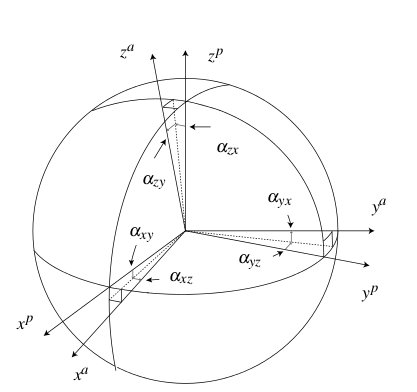
\includegraphics[width=0.5\textwidth]{./pics_acc/ejes_acc.jpg}
  \end{center}
  \vspace{-20pt}
  \caption{Rotaciones entre los ejes de la plataforma y del acelerómetro}
  \label{fig:ejes}
  \vspace{-10pt}
\end{figure}

Estos parámetros son constantes ya que su origen es puramente de construcción y se puede asumir que las orientaciones se mantendrán durante la vida útil del sensor.

\subsubsection*{Drift aleatorio y variación de las medidas con la temperatura}

La salida del acelerómetro es una tensión que luego es convertida a un nivel digital gracias a un conversor AD. Asumiendo un modelo lineal, la relación entre la aceleración y la medida realizada se puede expresar matricialmente de la siguiente forma:
 
$$\tilde{\mathbf{a}}^a = K_a \mathbf{a}^a + \mathbf{b}_a$$ donde $K_a$ es una matriz diagonal que representa el factor de escala para convertir del valor digital a una aceleración correspondiente. $\mathbf{b}_a$ no es otra cosa que un término independiente para corregir la posición del cero, que no necesariamente corresponde a la mitad de la escala digital. Estos dos parámetros poseen algunas de las fuentes de error que resulta más difícil de corregir. Resulta que dichos parámetros varían con la temperatura, por lo tanto se pueden observar algunas variaciones según la estación del año o el momento del día. A su vez, dichos parámetros poseen un drift aleatorio. 

Podemos pensar estos parámetros como un valor estático más un valor relativamente pequeño que varía según estas descripciones. 
En una primera instancia intentaremos caracterizar los valores estáticos.   

\subsubsection{Modelo del acelerómetro}

A partir del anális realizado se puede concluir que el modelo de acelerómetro que se considerará es el siguiente:

$$\tilde{\mathbf{a^a}}=K_a(T_a^p)^{-1}\mathbf{a^p}+b_a$$

\section{Procedimiento}
\subsection{Caracterización de las no idealidades variables}

Previo a la calibración de los parámetros estáticos parece interesante estudiar una serie ``larga" de muestras. En particular se tomará una hora de muestras a una tasa de muestreo de 50Hz. Estos datos serán útiles para la determinación de dos no idealidades:  
\begin{itemize}
\item Ruido inherente
\item Drift aleatorio
\end{itemize}

Además se realizará una medida variando la temperatura ambiente a fin de determinar la magnitud del Drift térmico.

\subsection{Determinación de parámetros estáticos}

Como se desprende de la sección anterior, para poder calibrar el acelerómetro se deben determinar 12 parámetros. Por dicho motivo, se precisan obtener al menos 12 ecuaciones diferentes. Típicamente se trabaja con el doble o triple de ecuaciones que de parámetros a determinar. Para mejorar los resultados se trabajará con 27 medidas donde cada una de ellas aporta 3 ecuaciones (una por cada eje), logrando un total de 81 ecuaciones, y se procederá a determinar los parámetros que minimizan el error cuadrático medio entre los valores efectivamente medidos y los valores teóricos. 

\subsubsection*{Preparación}
Para realizar una buena calibración es muy importante contar con una figura geométrica en forma de paralelepípedo de forma de poder solidarizar la IMU a dicho objeto. De esta forma nos aseguramos que no se introducen errores a la hora de orientar un eje en una dirección particular. Del mismo modo, es ideal disponer de una superficie perpendicular a la vertical y otra paralela, de modo que para rotar 90 grados la IMU, basta con rotar el paralelepípedo ese mismo ángulo, es decir, apoyar otra de las caras del mismo. \\

\begin{wrapfigure}{r}{0.5\textwidth}
  \vspace{-20pt}
  \begin{center}
    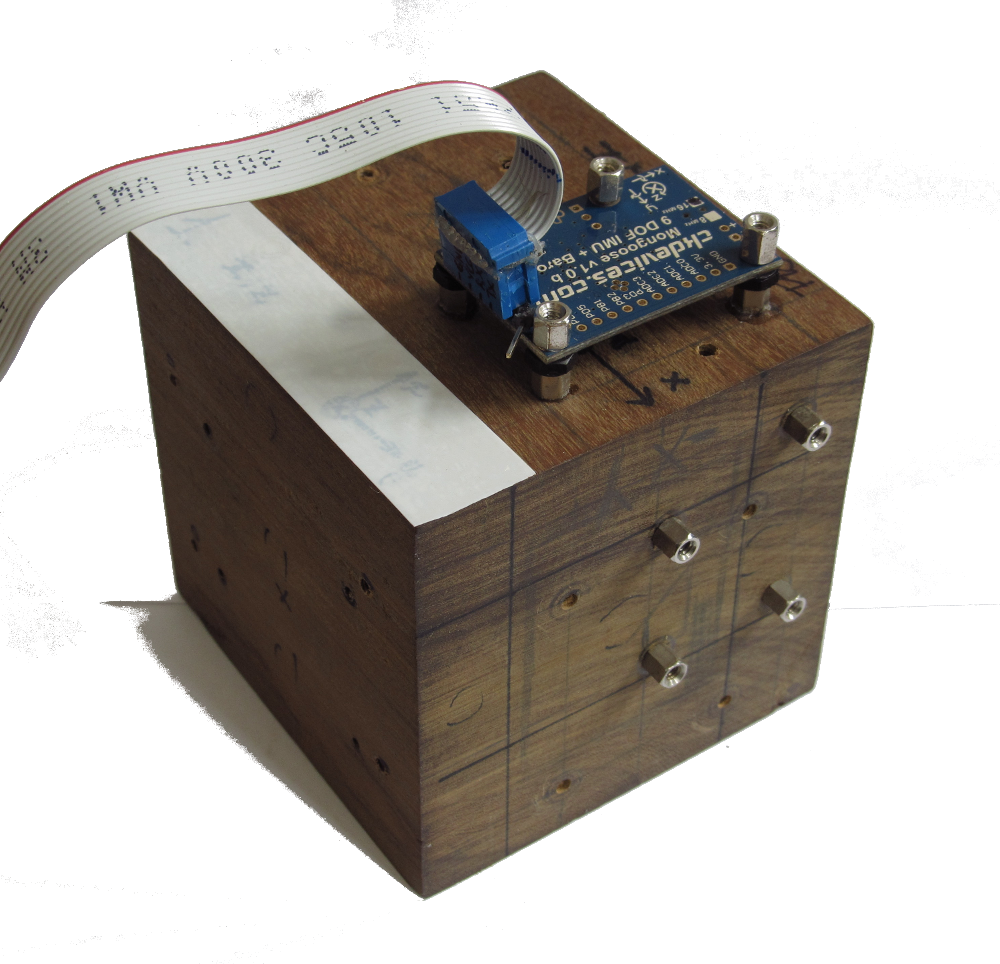
\includegraphics[width=0.42\textwidth]{./pics_acc/cubo.png}
  \end{center}
  \vspace{-20pt}
  \caption{Cubo de lapacho}
  \label{fig:cubo}
\end{wrapfigure}

El prisma que se utilizó fue el cubo de lapacho que puede verse en la figura \ref{fig:cubo}. \\
Los ángulos del mismo son prácticamente rectos difiriendo a lo sumo en medio grado. \\

Se construyo una plataforma de madera en forma de mesa con la tapa superior móvil, de modo que permite el giro sobre uno de sus lados (eje de giro). Se muestra en la figura \ref{fig:mesa-flotando}.  A su vez, es posible ajustar el dispositivo de forma de asegurar que dicho eje se encuentre en posición horizontal, por medio de 3 patas de altura regulable situadas en la parte inferior de la mesa. Para realizar las 27 medidas se irá modificando el ángulo de la tapa móvil de la plataforma y será medido con un semicírculo solidarizado a dicha tapa y un péndulo. En cada posición de la plataforma se tomarán medidas colocando el cubo en 3 posiciones distintas.

\begin{figure}[h!]
	\begin{center}
		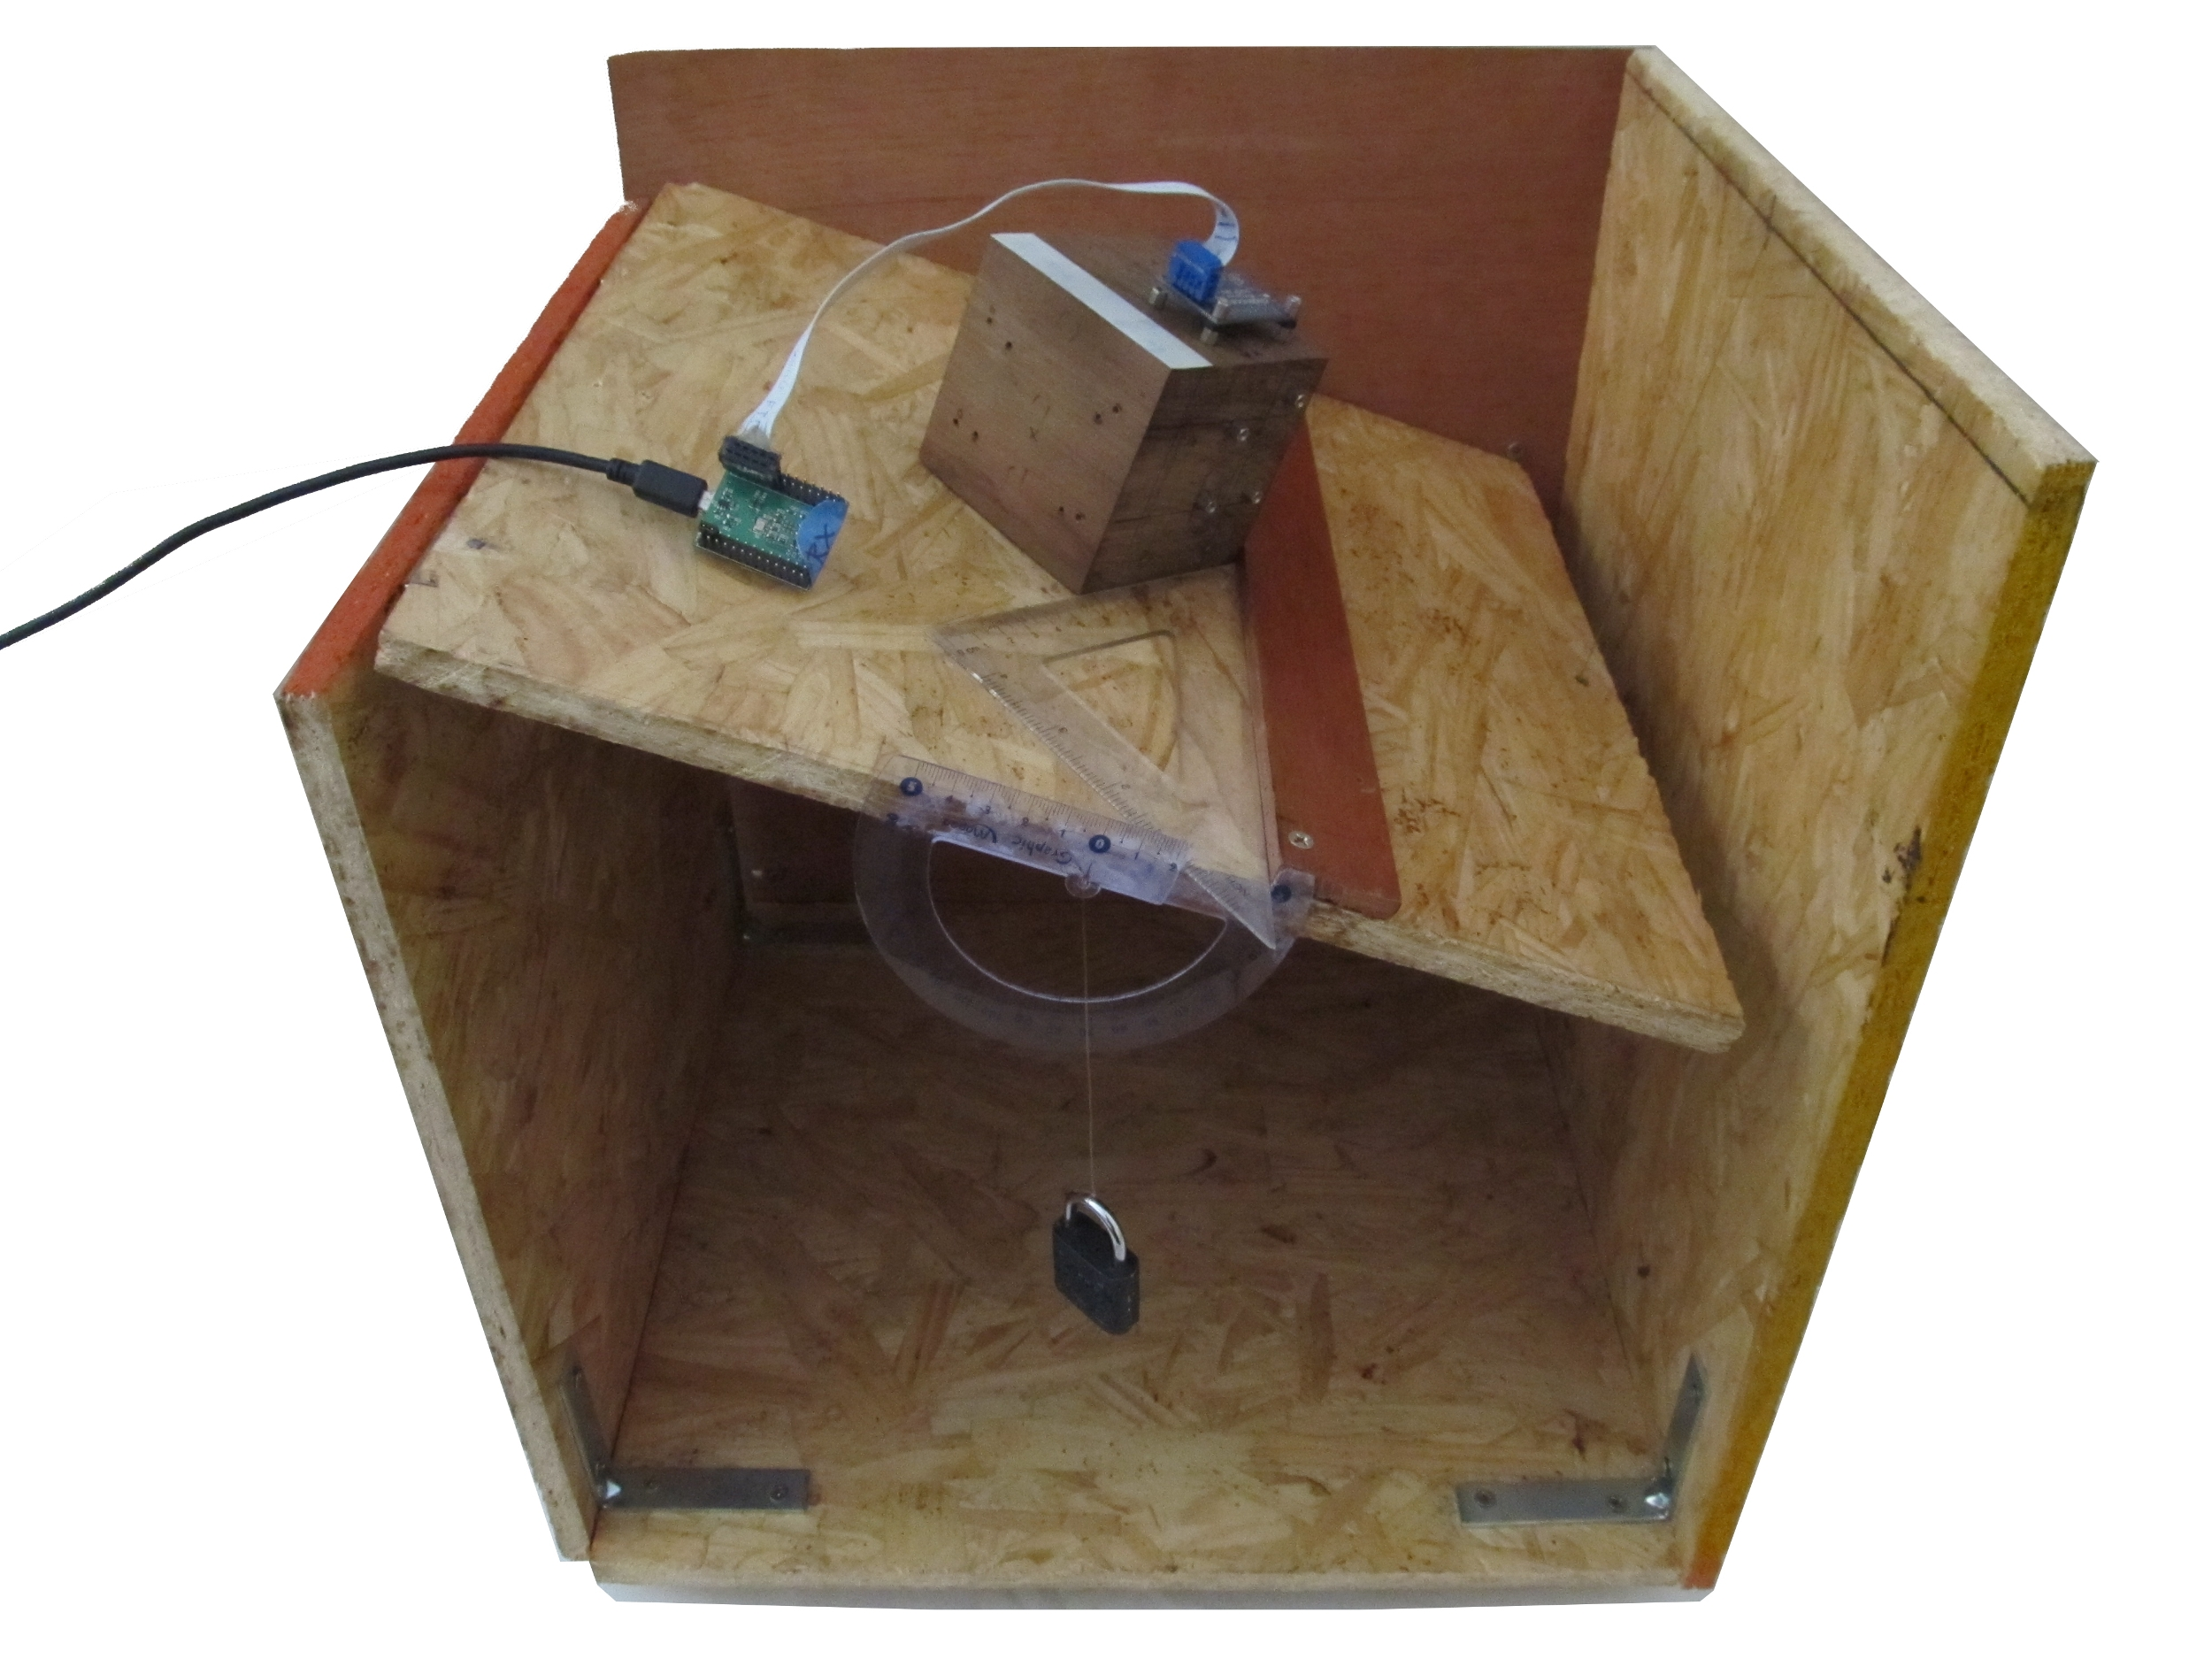
\includegraphics[width=0.7\textwidth]{./pics_acc/mesa-flotando.jpg}
	\end{center}
	\vspace{-20pt}
	\caption{Mesa - Plano inclinado regulable}
	\label{fig:mesa-flotando}
\end{figure}

\subsubsection*{Medidas a realizar}
En reposo el acelerómetro medirá una fuerza igual a \textit{g} en la dirección vertical y en el sentido radial saliente de la Tierra. En cada uno de los ejes de sensibilidad del acelerómetro se medirá la proyección ortogonal de dicho vector gravedad sobre cada eje. De esta forma, con distintas orientaciones se obtendrá una descomposición distinta.

\section{Resultados y análisis}
\subsection{Medida estática durante una hora}

En la figura \ref{fig:1hora} pueden observarse los datos crudos obtenidos de las aceleraciones registradas en los tres ejes de la IMU durante un período de 1 hora.

\begin{figure}[h!]
%  \vspace{-20pt}
  \begin{center}
    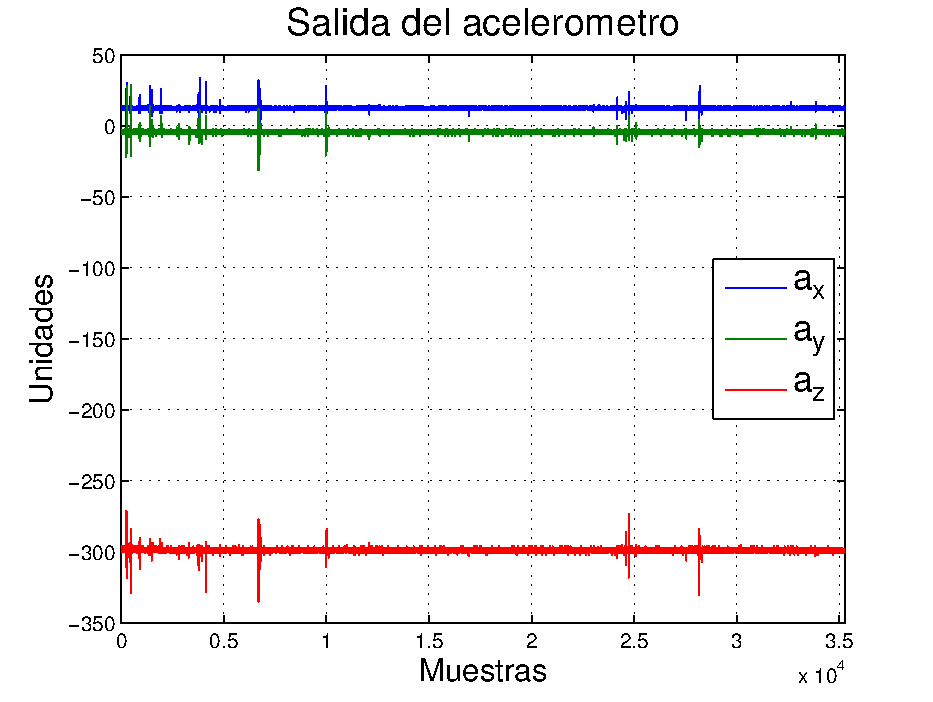
\includegraphics[width=0.8\textwidth]{./pics_acc/1hora.pdf}
  \end{center}
  \vspace{-20pt}
  \caption{Aceleraciones y velocidades angulares registradas por la IMU orientada con el eje z verticalmente y en reposo}
  \label{fig:1hora}
%  \vspace{-10pt}
\end{figure}

Se observa que dos medidas corresponden a un valor cercano a 0, mientras que la aceleración medida en z es cercana a -300. El eje z es el ubicado verticalmente hacia abajo, por lo tanto en dicha dirección se debería leer una medida equivalente a $-g$, mientras que en los otros dos ejes se debería leer un valor que corresponde a aceleración cero. Más allá de estas consideraciones, que permiten simplemente demostrar cierta coherencia entre lo esperado y lo obtenido,podemos afirmar que el ruido observado es asociable a un ruido blanco de media nula. Por otra parte no parece haber una deriva en las medidas realizadas. 

A partir de dichas constataciones se podrá afirmar que trabajar con el valor promedio de una tirada de medidas arrojará un resultado muy similar al que se obtendría trabajando con la tirada completa. 


\subsection{Medias estáticas para el acelerómetro}

Como se aclaró en la sección anterior se trabajará con el promedio de las aceleraciones medidas en una serie de datos. Cada serie de datos es de 20 segundos de duración. Además de variar el ángulo ($\theta$) de la mesa, se rotará el prisma de forma de realizar una medida con cada eje perpendicular al plano de la mesa. Asimismo utilizando una escuadra se lograrán rotaciones de 45º respecto del eje perpendicular a la tapa ($\phi$). Los resultados obtenidos se presentan en la tabla \ref{tab:acc}. Se utiliza la siguiente notación para las orientaciones utilizadas:
\begin{itemize}
	\item Orientación ``z''
	\begin{itemize}
		\item Eje ``z'' perpendicular a la tapa de la mesa y hacia abajo.
		\item Giro de la tapa de la mesa según el eje ``x''.
	\end{itemize}
	\item Orientación ``y''
	\begin{itemize}
		\item Eje ``y'' perpendicular a la tapa de la mesa y hacia abajo.
		\item Giro de la tapa de la mesa según el eje ``-z''.
	\end{itemize}
	\item Orientación ``x''
	\begin{itemize}
		\item Eje ``x'' perpendicular a la tapa de la mesa y hacia arriba.
		\item Giro de la tapa de la mesa según el eje ``y''.
	\end{itemize}
\end{itemize}
El tercer eje se deduce sabiendo que la base es directa. La aceleración medida es un número sin unidades.

\begin{table}[H]
\centering
\begin{tiny}
\begin{tabular}{p{30pt}p{30pt}|p{40pt}|p{26pt}|p{40pt}|p{26pt}|p{40pt}|p{26pt}|}
\hhline{~~------}
&

& \multicolumn{2}{|p{79pt}|}{\cellcolor[gray]{0.5} \centering \textbf{Orientación z}}  
& \multicolumn{2}{|p{79.5pt}|}{\cellcolor[gray]{0.5} \centering \textbf{Orientación x}}
& \multicolumn{2}{|p{78.7pt}|}{\cellcolor[gray]{0.5} \centering \textbf{Orientación y}} \\ \hline 

  \multicolumn{2}{|p{72.5pt}|}{\cellcolor[gray]{0.6}  \centering\textbf{Posición}}  
& \multicolumn{6}{|p{262.8pt}|}{\cellcolor[gray]{0.6} \centering\textbf{Aceleraciones}}  \\ \hline
  \multicolumn{1}{|p{30pt}|}{\cellcolor[gray]{0.7} $\theta(º)$}
& \multicolumn{1}{|p{30pt}|}{\cellcolor[gray]{0.7} $\phi(º)$} 
& \multicolumn{1}{|p{40pt}|}{\cellcolor[gray]{0.8} \textbf{Medida}}  
& \multicolumn{1}{|p{26.2pt}|}{\cellcolor[gray]{0.7} Teórica ($ms^{-2})$ }
& \multicolumn{1}{|p{40pt}|}{\cellcolor[gray]{0.8} \textbf{Medida}}  
& \multicolumn{1}{|p{26.7pt}|}{\cellcolor[gray]{0.7} Teórica ($ms^{-2})$ }
& \multicolumn{1}{|p{40pt}|}{\cellcolor[gray]{0.8} \textbf{Medida}}  
& \multicolumn{1}{|p{26pt}|}{\cellcolor[gray]{0.7} Teórica ($ms^{-2})$ }
\\ \hline
\multicolumn{1}{|p{30pt}|}{0}  & 0  &  16.18138;    0.3579454;    -296.1701 &       0;          0;      -9.81 & 276.9511;      -0.3572594;    -46.29364 &   9.81;          0;         0 & 13.39179;    -266.4408;    -44.0221 &      0;      -9.81;         0\\ \hline
\multicolumn{1}{|p{30pt}|}{10} & 0  &  16.27273;    -49.02392;     -292.201 &       0;    -1.7035;     -9.661 & 272.6542;       -0.045677;    0.5318108 &  9.661;          0;    1.7035 & 61.69231;    -262.3715;    -44.1195 & 1.7035;     -9.661;         0\\ \hline
\multicolumn{1}{|p{30pt}|}{10} & 45 & -14.74318;    -35.02247;    -292.0225 & -1.2045;    -1.2045;     -9.661 & 272.8368;        -33.2294;    -12.55412 &  9.661;    -1.2045;    1.2045 & 48.10742;    -262.3444;    -11.9763 & 1.2045;     -9.661;    1.2045\\ \hline
\multicolumn{1}{|p{30pt}|}{20} & 0  &  16.74718;    -94.71498;    -279.7955 &       0;    -3.3552;    -9.2184 & 260.3108;     -0.01932367;     43.84863 & 9.2184;          0;    3.3552 & 107.4279;    -251.4245;    -44.0647 & 3.3552;    -9.2184;         0\\ \hline
\multicolumn{1}{|p{30pt}|}{20} & 45 &   -48.512;     -66.7136;    -278.9184 & -2.3725;    -2.3725;    -9.2184 & 260.2182;       -65.37851;     18.87273 & 9.2184;    -2.3725;    2.3725 & 79.13748;    -251.2897;     19.3682 & 2.3725;    -9.2184;    2.3725\\ \hline
\multicolumn{1}{|p{30pt}|}{30} & 0  &  16.37318;    -136.5687;    -259.0533 &       0;     -4.905;    -8.4957 & 242.0839;    -0.004746835;     85.09968 & 8.4957;          0;     4.905 & 149.6053;    -229.7778;    -42.7181 &  4.905;    -8.4957;         0\\ \hline
\multicolumn{1}{|p{30pt}|}{30} & 45 & -76.82085;    -96.91368;    -259.6808 & -3.4684;    -3.4684;    -8.4957 & 242.3039;       -95.85131;     48.34477 & 8.4957;    -3.4684;    3.4684 & 109.3377;    -230.7721;      48.941 & 3.4684;    -8.4957;    3.4684\\ \hline
\multicolumn{1}{|p{30pt}|}{45} & 0  &  15.07717;    -190.8315;    -220.3402 &       0;    -6.9367;    -6.9367 & 198.5261;      0.07394958;      136.558 & 6.9367;          0;    6.9367 & 200.7626;    -189.0423;    -42.6423 & 6.9367;    -6.9367;         0\\ \hline
\multicolumn{1}{|p{30pt}|}{45} & 45 & -117.0878;    -134.7984;    -219.9024 &  -4.905;     -4.905;    -6.9367 & 198.4038;       -133.7997;     84.62754 & 6.9367;     -4.905;     4.905 & 145.8022;    -188.9018;     85.0561 &  4.905;    -6.9367;     4.905\\ \hline


\end{tabular}
\caption{Aceleraciones medidas y aceleraciones teóricas en los tres ejes de la plataforma}
\label{tab:acc}
\end{tiny}
\end{table} 

Para la calibración se consideran solamente 24 de las 27 medidas realizadas a fin. Esto es útil ya que se tienen 3 medidas que no serán tenidas en cuenta en la calibración para realizar una verificación de qué tan buena es la calibración obtenida.

El problema de calibración consiste en encontrar el vector de parámetros $\theta$ que mejor ajusta las medidas obtenidas a los valores teóricos de aceleración. El vector $\theta$ se compone de los elementos de la diagonal de la matriz $K_a$, de los elementos de $b_a$ y de los $\alpha_{ij}$ de la matriz $T_a^p$. Es decir: $$\theta =\left[ k_{ax} , k_{ay} , k_{az} ,b_{ax} ,b_{ay} ,b_{az}, \alpha_{yz} , \alpha_{zy} , \alpha_{xz} , \alpha_{zx} , \alpha_{xy} , \alpha_{yx} \right]$$

Como criterio de ajuste se decide minimizar la suma de los cuadrados de las diferencia entre la aceleración teórica y la aceleración medida. Dicho problema se puede expresar matemáticamente como:

$$\theta \quad : \quad  min \left\lbrace \sum_{i=1}^{M} {\vert \vert\tilde{\mathbf{a}}_{i}^p-T_a^pK_a^{-1}\left(\tilde{\mathbf{a}}_{i}^a -\mathbf{b}_a \right)\vert \vert} \right\rbrace$$
donde M es la cantidad de medidas realizadas, $\tilde{\mathbf{a}}_{i}^p$ los valores de aceleración teóricos en cada eje de la plataforma según la posición y orientación de la IMU y $\tilde{\mathbf{a}}_{i}^a$ los valores obtenidos de la IMU.
Las relaciones entre los parámetros a determinar $\mathbf{no}$ es lineal, por lo tanto se utilizará para su determinación un algoritmo de mínimos cuadrados no lineales. \emph{Matlab}  provee un algoritmo con dicho fin: \emph{lsqnonlin}. El algoritmo precisa además una semilla para comenzar, dicha semilla debe ser bien elegida de forma de que el mínimo encontrado por el algoritmo sea el deseado. Sucede que dicho algoritmo encuentra mínimos locales. Si la semilla proporcionada se encuentra muy lejos de la solución que en realidad interesa, se puede obtener una solución que no sirva. \\

El rango de aceleraciones manejado en la prueba es de $\pm 16g$. Según la hoja de datos del acelerómetro, se tiene una ganancia de $3.9 mg/LDB$. La ganancia debe ser entonces $\frac{1}{g \times 3.9 \times 10^{-3}}=26.1376$ para los tres ejes. La IMU expresa las aceleraciones obtenidas en complemento a2, por lo que una aceleración de 0 equivale a una lectura de 0. Finalmente, los ángulos se suponen pequeños, por lo tanto una semilla válida parece ser: 
$$\theta_0=\left[ \frac{1}{g \times 3.9 \times 10^{-3}}, \frac{1}{g \times 3.9 \times 10^{-3}}, \frac{1}{g \times 3.9 \times 10^{-3}}, 0, 0, 0, 0, 0, 0, 0, 0, 0 \right]$$

Los parámetros que minimizan la suma de los errores al cuadrado son los siguientes:

\begin{scriptsize}
$$\theta=\left[ 26.9553 \quad 27.1044 \quad 25.9160 \quad 13.0717 \quad -1.0795 \quad -40.7236 \quad -0.0095 \quad 0.0096 \quad -0.0004 \quad 0.0068 \quad -0.0105 \quad -0.0046 \quad \right]$$
\end{scriptsize}

Luego de realizada la minimización se calcula la media del error cometido y la desviación estándar del error.
$$\mu=6.88 \times 10^{-10} ms^{-2}$$ \\
$$\sigma =  0.0397 ms^{-2}$$ 
 
La media del error cometido es completamente despreciable, por lo tanto podemos afirmar que el $95\% $ de las medidas de aceleración realizadas tendrán un error inferior $2\sigma=0.0794$. Este error se integrará dos veces a la hora de obtener la posición del cuadricóptero, por lo tanto en el $95 \%$ de los casos estaremos cometiendo un error inferior a los 5 metros al cabo de 10 segundos de navegación. 
 
Para verificar la calibración realizada se utilizan las medidas siguientes:
\begin{itemize}
\item $\theta = 0 \quad \phi = 0 \quad$ orientación z
\item $\theta = 20 \quad \phi = 0 \quad$ orientación x
\item $\theta = 10 \quad \phi = 45 \quad$ orientación y
\end{itemize}

Se presenta para las tres medidas la aceleración teórica, la medida convertida con los parámetros obtenidos y el error en la tabla \ref{tab:diff}. 

\begin{table}[H]
\centering
\begin{tabular}{|p{90pt}|p{90pt}|p{90pt}|p{90pt}|}
\hline
\cellcolor[gray]{0.8}{Medida} & \cellcolor[gray]{0.8}{Aceleración Medida ($ms^{-2}$)}&\cellcolor[gray]{0.8}{Aceleración teórica($m^{-2}$)}& \cellcolor[gray]{0.8}{Error($ms^{-2}$)} \\
\hline
1 &  0.0217; 0.120; -9.856   & 0.00;0.00;-9.810     & 0.0217; 0.120; -0.0460\\
\hline
2 & 9.204;0.0136;3.359       & 9.218;0.00;3.355     & -0.0140; 0.0136; 0.00400\\
\hline
3 & 1.218;-9.647;1.167       & 1.204;-9.660;1.205   & 0.0140; 0.0130 -0.0380\\
\hline
\end{tabular}
\caption{Medidas de verificación}
\label{tab:diff}
\end{table}

Si bien estos valores no son una buena muestra estadística, sirven como verificación ya que en la mayoría de los casos se obtiene un error inferior a $\sigma$ y tenemos solamente un error superior a $2\sigma$.

\subsection{Variación con la temperatura}

\begin{figure}[H]
  \begin{center}
    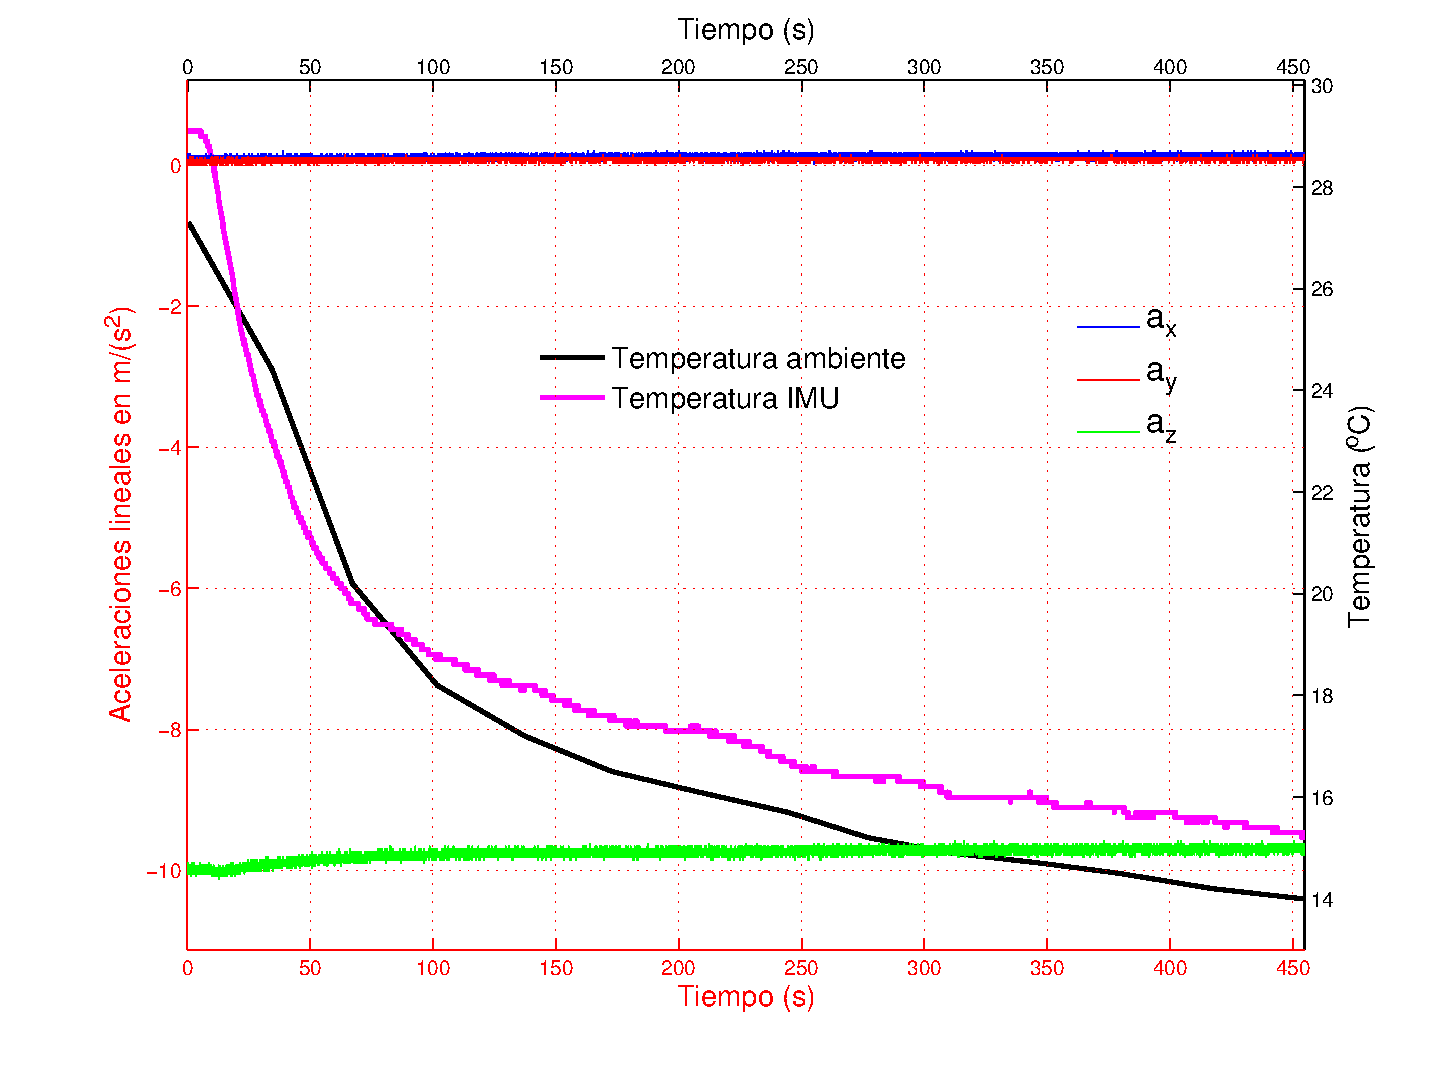
\includegraphics[width=0.8\textwidth]{./pics_acc/bajada.pdf}
  \end{center}
  \vspace{-20pt}
  \caption{Variación de la medida del acelerómetro con la temperatura }
  \label{fig:bajada}
\end{figure}

\subsection{Análisis de variación}
A partir del análisis de los experimentos realizados es claro que la mínima variación existente en las señales procedentes de los acelerómetros es del orden de $0.04 m/s^2$, tal como puede observarse en la siguiente gráfica:

\begin{figure}[H]
  \begin{center}
    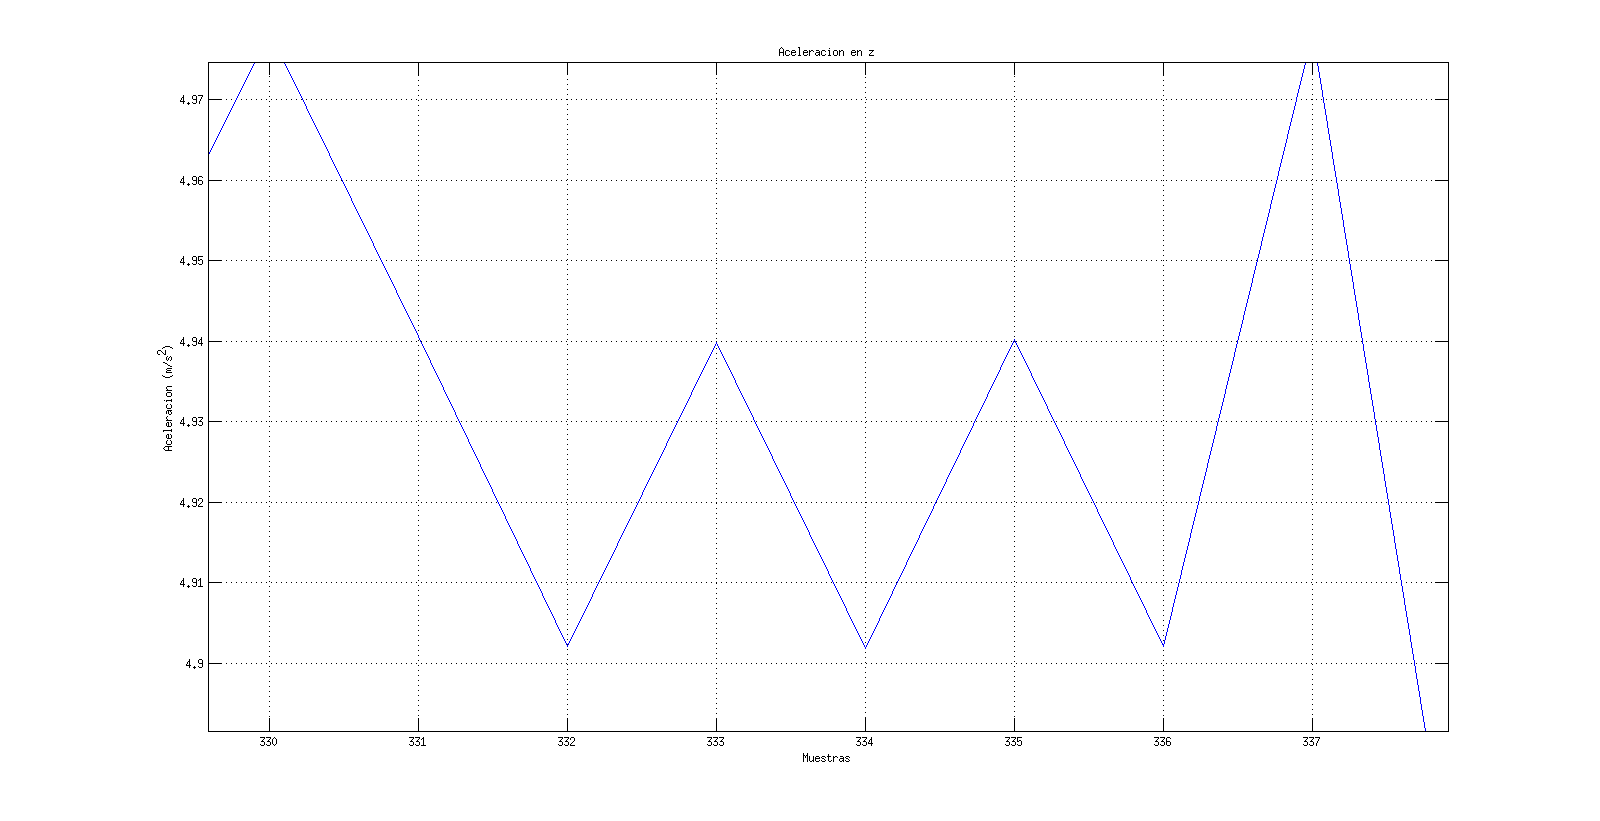
\includegraphics[width=0.8\textwidth]{./pics_acc/variacion.png}
  \end{center}
  \vspace{-20pt}
  \caption{Variación de la medida del acelerómetro con la temperatura }
  \label{fig:variacion}
\end{figure}

Por otro lado, de los parámetros obtenidos de la calibración, se determina que $\sigma= 0.0396798455378608$, lo cual resulta coherente con el resultado anterior.\\
\\
Finalmente, de la hoja de datos del acelerómetro se obtiene que el factor de escala para la señal es de $3.9 mg/LSB$, lo cual nuevamente es coherente con los resultados obtenidos anteriormente.\\
\\
De lo anterior puede concluirse que el procedimiento de calibración parecería ser correcto, obteniéndose valores similares para $\sigma$ tanto en la teoría como en la realidad.
\end{document}